\chapter{GTFS}
\label{2-teorie-gtfs}

General Transit Feed Specification, zkráceně GTFS, je dokument, který definuje
obecný formát pro jízdní řády veřejné dopravy a příbuzné geografické informace.
GTFS „feeds“ umožňují veřejným dopravním agenturám zveřejňovat svá přepravní
data a vývojářům psát aplikace, které tato data spotřebovávají interoperabilním
způsobem. \cite{gtfs-info}

GTFS dataset obsahuje CSV soubory, jehož úplný seznam je v následující tabulce. Co to jsou CSV soubory?

CSV, \textit{Comma-separated values}, v překladu \textit{hodnoty oddělené čárkami}, je jednoduchý 
souborový formát určený pro výměnu tabulkových dat. Data jsou oddělována „oddělovačem“.
Ačkoli podle definice by měl být formát oddělen čárkami, oddělovač může být prakticky cokoli. 
Nejčastějšími oddělovači jsou právě čárky, středníky nebo mezery. CSV soubor se 
může upravovat v jakémkoliv textovém editoru.
\begin{figure}[H] \centering
    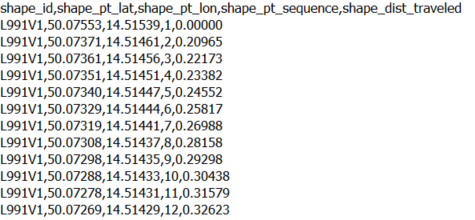
\includegraphics[width=250pt]{./pictures/ukazka-csv.PNG}
    \caption[Ukázka CSV formátu ze souboru shapes.txt]{Ukázka CSV formátu ze souboru shapes.txt}
	\label{fig:ukazka-csv}              
\end{figure}


\begin{figure}[H] \centering
    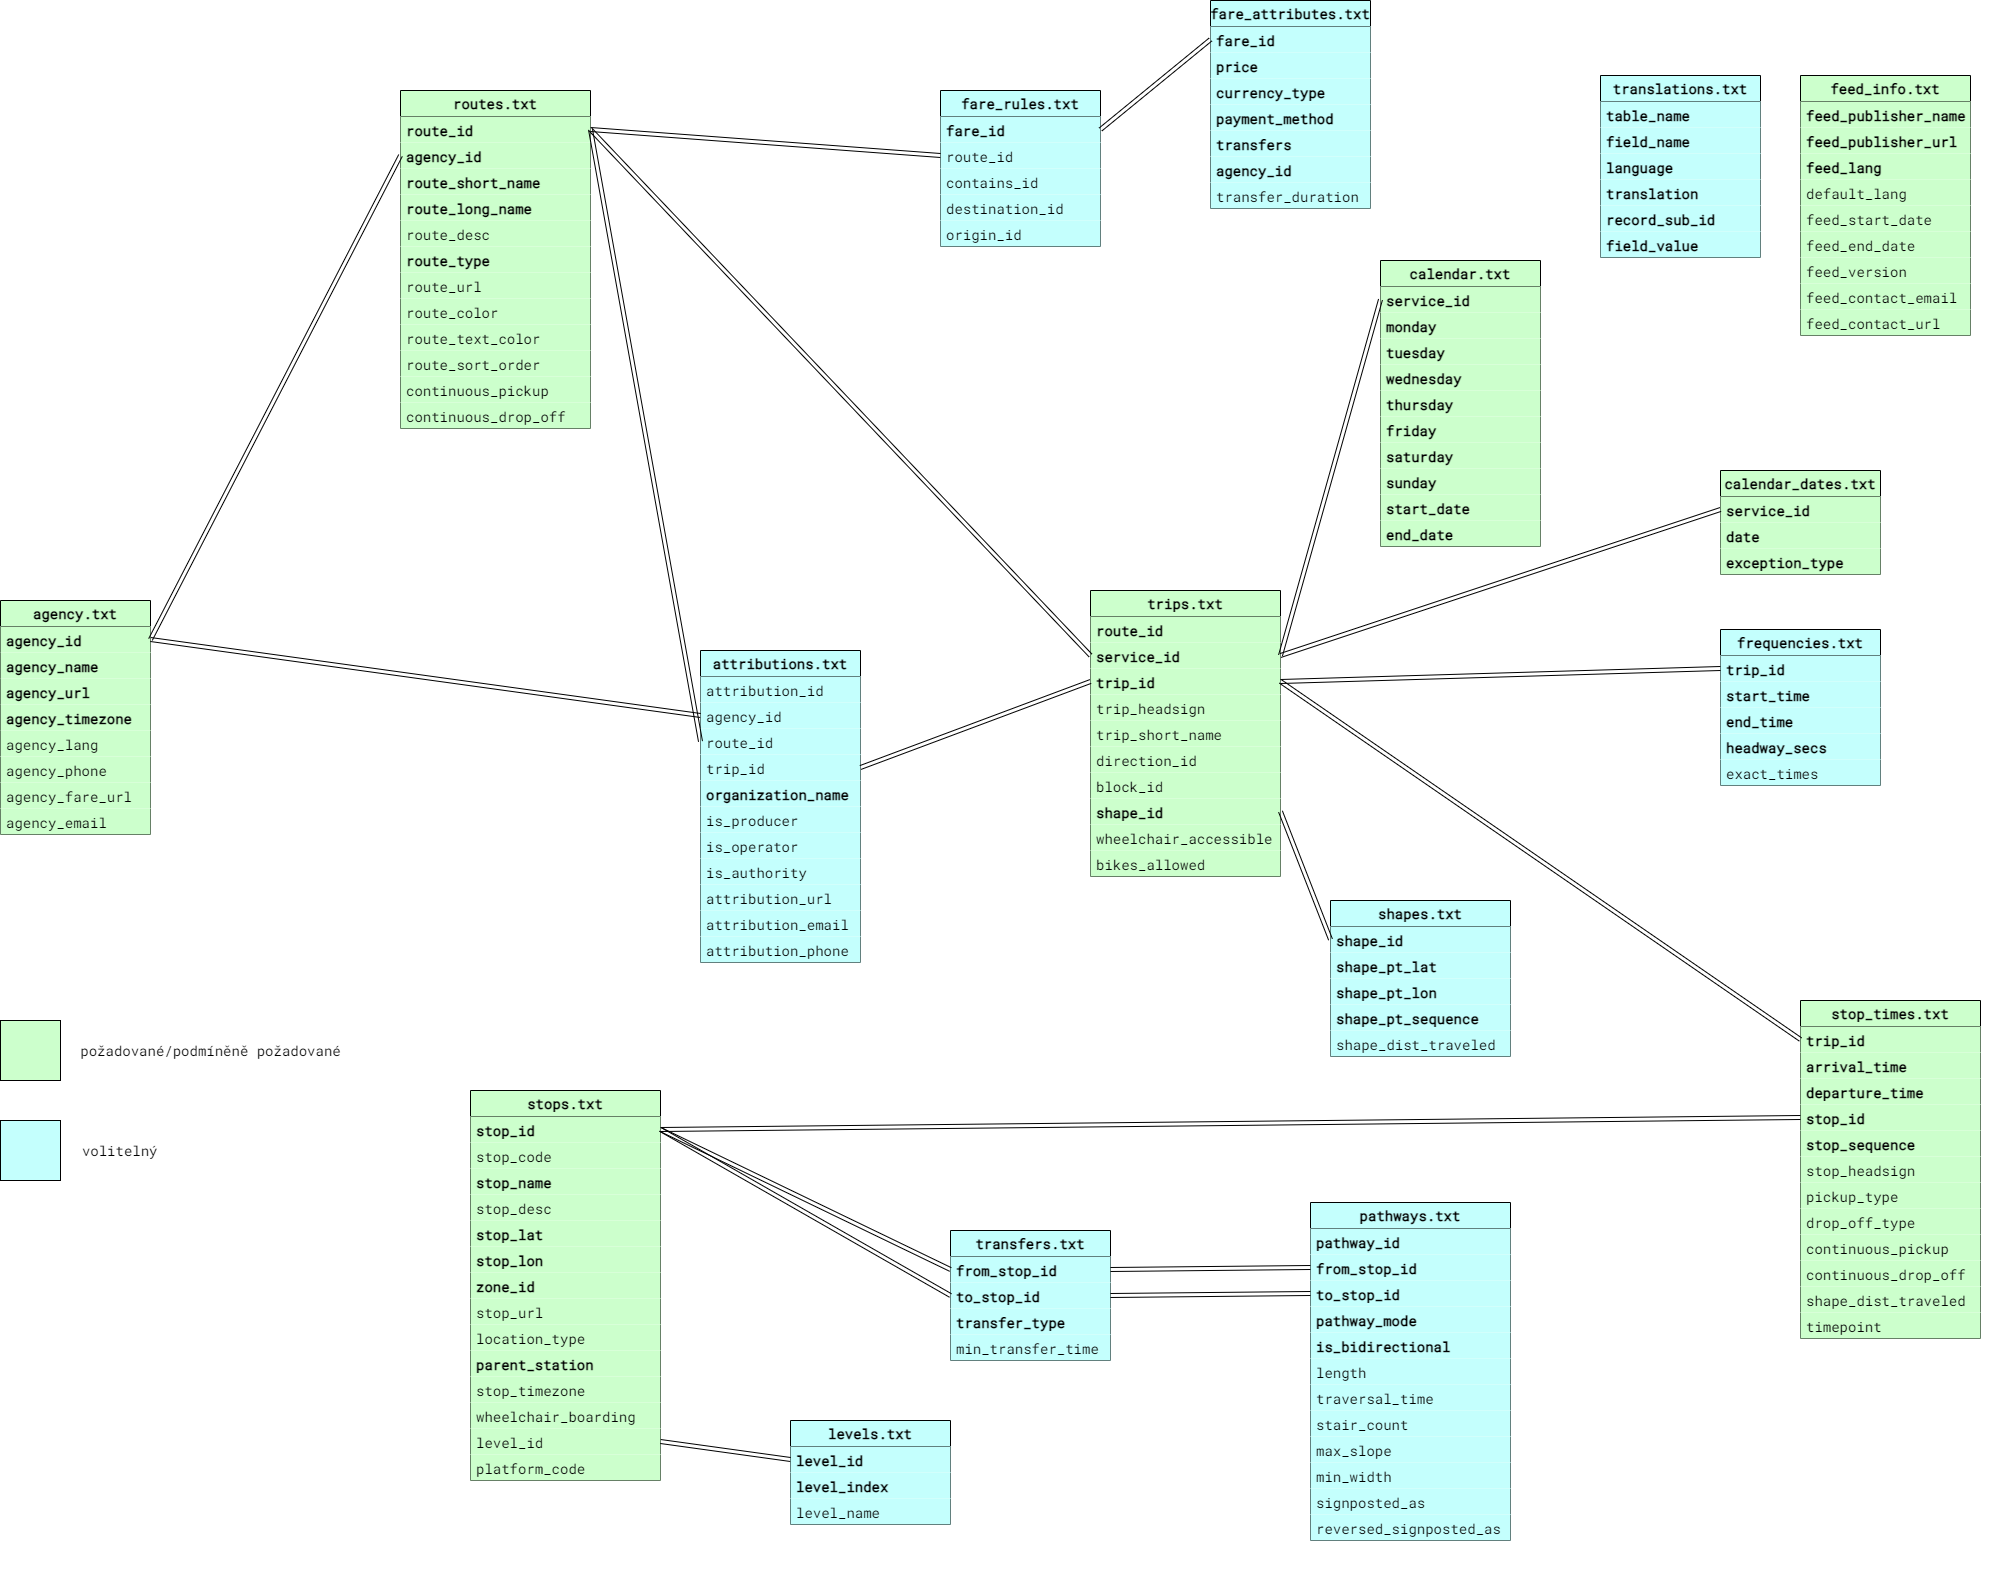
\includegraphics[width=400pt]{./pictures/GTFS-diagram.PNG}
    \caption[Diagram GTFS datasetu]{Diagram GTFS datasetu}
	\label{fig:GTFS-diagram}              
\end{figure}
